%================================================================================
% Implicit Solvent Parametrisation by Force Matching
% Jens Kleinjung and Franca Fraternali
% ISMB 2016 Orlando
% poster
%================================================================================

\documentclass{beamer}
\usepackage[orientation=portrait,size=a0,scale=1.4,debug]{beamerposter}
\mode<presentation>{\usetheme{FC}}
\usepackage{caption}
\usepackage[utf8]{inputenc}
\usepackage[english]{babel}
\usepackage{siunitx} % pretty measurement unit rendering
\usepackage{hyperref} % enable hyperlink for urls
\usepackage{ragged2e}
\usepackage{calc}
\newlength{\mylength}
\usepackage{array,booktabs,tabularx}
\newcolumntype{Z}{>{\centering\arraybackslash}X} % centered tabularx columns
\newcommand{\sig}{$\sigma_i^{SASA}$}
\newcommand{\gam}{$\gamma_i^0$}
\captionsetup[figure]{name=Fig.}
\captionsetup[table]{name=Eq. for Fig. }
%______________________________________________________________________________
\title{\huge Implicit Solvent Parametrisation by Force Matching}
\author{Jens Kleinjung and Franca Fraternali}
\institute[]{The Francis Crick Institute, King's College London}
\date{\today}
\newlength{\columnheight}
\setlength{\columnheight}{105cm}
%______________________________________________________________________________
\begin{document}
\begin{frame}
\begin{columns}
\begin{column}{.45\textwidth}
\begin{beamercolorbox}[center]{postercolumn}
\begin{minipage}{.98\textwidth}  % tweaks the width, makes a new \textwidth
\parbox[t][\columnheight]{\textwidth}{ % must be some better way to set the the height, width and textwidth simultaneously
%______________________________________________________________________________
\begin{myblock}{Introduction}
Molecular dynamics simulations of biomolecules are routinely performed in
a water box with periodic boundary conditions. While the explicit representation
of water molecules provides a high level of detail in regard to solute-solvent
interactions, treating their degrees of freedom becomes gradually prohibitive
with increasing system size. For systems whose detailed water interactions are
not relevant to the properties under study, implicit solvation is a suitable
method to represent the solvent-solute interactions \cite{Kleinjung_2014}.
\end{myblock}\vfill
%______________________________________________________________________________
\begin{myblock}{SASA Model}
The interaction potential $V^{impl}$ between the solvent and all solute
atoms $i$ can be assumed to be proportional to its solvent accessible
surface area (SASA), scaled by an atom-specific energy term \sig:
\begin{equation}
\label{eq:sasapot}
V^{impl}(\mathbf{r}^N) \; = \; \sum_{i=1}^{N} \, \sigma_i^{SASA} \, A_i(\mathbf{r}^N) \; .
\end{equation}
The implicit solvent forces per atom are obtained from the derivative of the above
equation with respect to $r_i$:
\begin{equation}
\label{eq:Fimpl}
\mathbf{f}_i^{impl} \; = \; - \, \sigma_i^{SASA} \, \frac{\partial A_i(\mathbf{r}^N)}{\partial \mathbf{r}_i} \; .
\end{equation}
\end{myblock}\vfill
%______________________________________________________________________________
\begin{myblock}{Force Matching}
\begin{figure}
\begin{minipage}{0.45\textwidth}
	\centering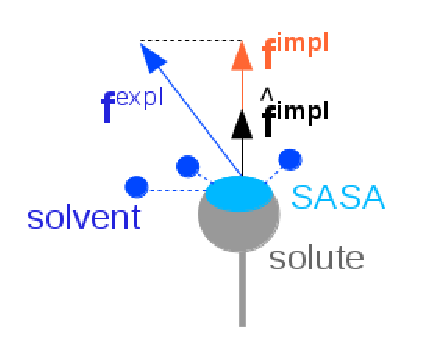
\includegraphics[width=1.0\textwidth]{./force_matching1.eps}
	\caption{Force matching: Explicit solvent forces (blue arrow) exerted on the solute are projected on the normal of its SASA (black arrow), yielding the implicit solvent force (orange arrow).}
\label{fig:projection}
\end{minipage}
%______________________________________
\begin{minipage}{0.45\textwidth}
\begin{gather}
	\label{eq:sigma}
	\nonumber \quad \\
	\left| \mathbf{f}_i^{impl} \right| \; = \; \hat{\mathbf{f}}_i^{impl} \; \cdot \; <\mathbf{f}_i^{expl}> \\
	\nonumber \quad \\
	\sigma_i^{SASA} \; = \; - \, \frac{ \frac{ \partial A_i} { \partial \mathbf{r}_i} }
		{\left| \frac{ \partial A_i} { \partial \mathbf{r}_i} \right| ^2 }
			\, \cdot \, <\mathbf{f}_i^{expl}>
\end{gather}
\begin{table}
\caption{Using the concept of force projection shown left,
the expression for \sig{} combines the observed forces in explicit
solvent with the derivative of the atomic SASA.}
\end{table}
\end{minipage}
\end{figure}
\end{myblock}\vfill
%______________________________________________________________________________
\begin{myblock}{\sig{} Parameters}
Using the solvation forces of 188 topologically diverse proteins in explicit
and implicit solvent, a robust set of \sig{} parameters was derived by
force matching \cite{Kleinjung_2012a}. Hydrophilic $N$ and $O$ atoms have
negative \sig{} parameters, those of hydrophobic $C$ atoms are positive.
\vspace{2cm}
\begin{figure}
\begin{minipage}{1.0\textwidth}
	\centering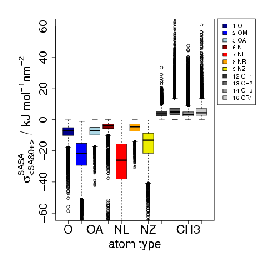
\includegraphics[width=0.7\textwidth]{./sigma.all.atomtype.box.sided.eps}
	\caption{\sig{} parameters derived by force matching.}
\label{fig:projection}
\end{minipage}
\end{figure}
\end{myblock}\vfill
%______________________________________________________________________________
\begin{myblock}{Friction}

\end{myblock}\vfill
%______________________________________________________________________________
\begin{myblock}{\gam{} Parameters}

\end{myblock}\vfill
%______________________________________________________________________________
\begin{myblock}{References}
\footnotesize
\bibliographystyle{abbrv}
\bibliography{./poster}
\end{myblock}\vfill
%______________________________________________________________________________
}\end{minipage}
\end{beamercolorbox}
\end{column}
\end{columns}
\end{frame}
\end{document}
%================================================================================

